\documentclass{article}
\usepackage{nips15submit_e}

\newcommand{\fix}{\marginpar{FIX}}
\newcommand{\new}{\marginpar{NEW}}
\usepackage{amssymb}
\usepackage{bm}
\usepackage{latexsym}
\usepackage{amsmath}
\usepackage{url}
\usepackage{graphicx}
\usepackage{hyperref}
\usepackage{hyperref}
\hypersetup{
    bookmarks=true,         
    unicode=true,  
    colorlinks=true,       
    linkcolor=blue,          
    citecolor=blue,       
    filecolor=blue,      
    urlcolor=blue          
}
\usepackage[ruled,vlined]{algorithm2e}
\usepackage{pstricks,pst-plot,pst-text,pst-tree,pst-eps,pst-fill,pst-node,pst-math}
\usepackage{caption}
\usepackage{subcaption}

\title{Latent Dirichlet allocation}
\author{
J\'er\^ome DOCK\`ES (\texttt{jerome@dockes.org}) \\
\textbf{Pascal LU (\texttt{pascal.lu@centraliens.net})} \\
\'Ecole Normale Sup\'erieure de Cachan \\
}

\begin{document}

\maketitle

We consider the problem of modeling text corpora. The goal is to find short descriptions of the members of a collection that enable efficient processing of large collections while preserving the essential statistical relationships. Our work is mainly based on \cite{BNJ03}.

\section{Latent Dirichlet allocation}
\subsection{Presentation of the model}

\textbf{Notations}
\begin{itemize}
\setlength\itemsep{-0.2em}
  \item $\mathcal{D} = \{d_{1},d_{2}, \ldots, d_{M}\}$ is a corpus (collection of $M=|\mathcal{D}|$ documents). We denote $|\mathcal{D}|$ (\verb"num_docs") the number of documents.
  \item $\mathcal{V}$ is the vocabulary. Its size is denoted $V$ (\verb"voc_size").
  \item The number of topics is denoted $k$ (\verb"num_topics").
\end{itemize}

For a document $d \in \mathcal{D}$,
\begin{itemize}  
\setlength\itemsep{-0.2em}
%  \item $d = (w_1, \ldots, w_{n(d)})$ represents the document $d$ of the corpus $^{(d)}$, composed of a sequence of $n(d)$ words.
  \item $d = (w_1^{(d)}, \ldots, w_{N_d}^{(d)})$ represents the document $d$. $N_d$ is the number of words in the document $d$.
  \item $w^{(d)}$ is a matrix whose element $w_{ni}^{(d)} = 1$ if the word $n$ in the 
document is the word $i$ in the vocabulary. The size of $w^{(d)}$ is $N_d \times V$.
  
 %   $w_{nj}^{(d)} = \begin{cases} 1 & \text{if the word in position } n \text{ of the document is the word in position } j \text{ of the dictionary} \\ 0 & \text{otherwise} \end{cases}$
 \item $\theta^{(d)}$ is an array of size $k$, representing a probability density.
 \item $z^{(d)}$ is the set of topics : $z_{ni}^{(d)} =  1$ if the word $n$ is linked with the topic $i$. Hence, it is a matrix of size $N_d \times k$.
\end{itemize}

\medskip

Latent Dirichlet allocation (LDA) is a generative probabilistic model of a corpus. The main idea is that documents are represented as random mixtures over latent topics, where each topic is characterized by a distribution over words. 

\begin{algorithm}
\caption{Generative process}
\KwResult{corpus $\mathcal{D}$}
\Begin{
\For{\emph{each document} $d \in \mathcal{D}$}{
Choose $N_d \sim \textnormal{Poisson}(\xi)$\;
Choose $\theta^{(d)} \sim \textnormal{Dir}(\alpha)$\;
\For{\emph{each of the $N_d$ words $w_n^{(d)}$}}{
Choose a topic $z_n^{(d)} \sim  \textnormal{Multinomial}(\theta^{(d)})$\;
Choose a word $w_n^{(d)}$ from $p(w_n^{(d)} |z_n^{(d)}, \beta)$, a multinomial probability conditioned on the topic $z_n^{(d)}$.
}
}
}
\end{algorithm}

\begin{figure}[ht!]
\begin{center}
\psset{xunit=1.0cm,yunit=1.0cm,algebraic=true,dimen=middle,dotstyle=o,dotsize=5pt 0,linewidth=0.8pt,arrowsize=3pt 2,arrowinset=0.25}
\begin{pspicture*}(-0.5,-0.3)(8,3.5)
\rput(0,1){\pscirclebox[linecolor=black,fillstyle=solid,fillcolor=blue]{\textcolor{white}{$\alpha_j$}}}
\rput(2,1){\pscirclebox{$\theta^{(d)}_j$}}
\rput(4,1){\pscirclebox{$z^{(d)}_{nj}$}}
\rput(6,1){\pscirclebox[linecolor=black,fillstyle=solid,fillcolor=yellow]{$w_{nj}^{(d)}$}}
\rput(6,3){\pscirclebox[linecolor=black,fillstyle=solid,fillcolor=blue]{\textcolor{white}{$\beta_{jv}$}}}
\pspolygon(3.25,0.25)(7.2,0.25)(7.2,1.75)(3.25,1.75)
\pspolygon(1.25,0)(7.75,0)(7.75,2)(1.25,2)
\psline{->}(0.33,1)(1.53,1)
\psline{->}(2.5,1)(3.53,1)
\psline{->}(4.5,1)(5.5,1)
\psline{->}(6,2.6)(6,1.52)
\rput(6.75,0.5){$N_d$}
\rput(7.5,0.25){$M$}
\end{pspicture*}
\caption{Generative model}
\label{generative}
\end{center}
\end{figure}

The following parameters are introduced:
\begin{itemize}
  \item $\alpha$ (\verb"dirich_param") is an estimate of the parameter of the dirichlet distribution which generates the parameter for the (multinomial) probability distribution over topics in the document. The size of $\alpha$ is the number of topics, $k$. \textbf{We suppose that $\alpha = \alpha \mathbf{1}_{k}$ (exchangeable Dirichlet distribution) \footnote{This assumption is suggested by the authors of \cite{BNJ03}.} .}
  
  \item $\beta$ (\verb"word_prob_given_topic") is a matrix of size (number of topics $\times$ vocabulary size $= k \times V$) which gives the (estimated) probability that a given topic will generate a certain word:
\[ \beta_{ij}= p(w^j = 1 | z^i = 1) \]
where $w^j$ the $j^{\text{th}}$ word of the vocabulary and $z^i$ the $i^{\text{th}}$ topic.
 \end{itemize}

LDA is based on the computation of the parameters $(\alpha, \beta)$, for instance by maximizing the log-likelihood. For a document $d$, the probability $p(d|\alpha, \beta)$ is given by:

\begin{align*}
p(d|\alpha, \beta) 
& = \int p(\theta^{(d)}|\alpha) \left( \prod_{n=1}^{N_{d}} p(w_n^{(d)}|\theta^{(d)}, \beta)\right) \text{d}\theta  \\
& = \int p(\theta^{(d)}|\alpha) \left( \prod_{n=1}^{N_{d}} \sum_{z_n^{(d)}} p(z_n|\theta^{(d)}) p(w_n^{(d)}|z_n^{(d)}, \beta)\right) \text{d}\theta  \\
& = \frac{\Gamma\left( \sum_i \alpha_i\right)}{\prod_i \Gamma(\alpha_i)} \int \left( \prod_{i=1}^k (\theta_i^{(d)})^{\alpha_i - 1} \right) \left( \prod_{n=1}^{N_d} \sum_{i=1}^k \prod_{j=1}^V (\theta_i^{(d)} \beta_{ij})^{w_{nj}^{(d)}} \right) \text{d}\theta
\end{align*}

\subsection{Inference and parameter estimation}

In the inference part, we need to compute the posterior distribution of the hidden variables given a document $d$:
\[ p(\theta^{(d)}, z^{(d)} | d, \alpha, \beta) = \frac{p(\theta^{(d)}, z^{(d)}, d | \alpha, \beta)}{p(d | \alpha, \beta)} \]

Unfortunately, the distribution $p(d|\alpha, \beta)$ is not computable in general.

The idea is to use Jensen's inequality to obtain an adjustable lower bound on the log likelihood and to introduce new latent variables.

For each document $d \in \mathcal{D}$, the following latent variables are introduced:
 \begin{itemize}
\setlength\itemsep{-0.2em}
  \item $\gamma^{(d)}$ (\verb"var_dirich") the variational parameter for the dirichlet distribution. The size of $\gamma^{(d)}$ is the number of topics, $k$.
  \item $\phi^{(d)}$ (\verb"var_multinom") the variational parameter for the multinomial distribution The size of $\phi^{(d)}$ is (number of distinct words in document $d$ $\times$ number of topics), $N_d \times k$.
  
  $\phi_{ni}^{(d)}$ depends on the relation between the word in position $n$ of the document and the topic $i$ of the list of topics.
   \end{itemize}

The conditional probability is $q(\theta^{(d)}, z^{(d)}|\gamma^{(d)}, \delta^{(d)}) = q(\theta^{(d)}|\gamma^{(d)}) \prod_{n=1}^{N_d} q(z_n^{(d)}|\phi_n^{(d)})$

\begin{figure}[ht!]
\begin{center}
\psset{xunit=1.0cm,yunit=1.0cm,algebraic=true,dimen=middle,dotstyle=o,dotsize=5pt 0,linewidth=0.8pt,arrowsize=3pt 2,arrowinset=0.25}
\begin{pspicture*}(-1,-0.1)(4,5)
\rput(0,3){\pscirclebox[linecolor=black,fillstyle=solid,fillcolor=green]{$\gamma^{(d)}_j$}}
\rput(0,1){\pscirclebox{$\theta^{(d)}_j$}}
\rput(2,3){\pscirclebox[linecolor=black,fillstyle=solid,fillcolor=green]{$\phi^{(d)}_{nj}$}}
\rput(2,1){\pscirclebox{$z^{(d)}_{nj}$}}
\pspolygon(1.25,0.25)(3.15,0.25)(3.15,3.75)(1.25,3.75)
\pspolygon(-0.9,0)(3.8,0)(3.8,4)(-0.9,4)
\psline{->}(0,2.5)(0,1.5)
\psline{->}(2,2.5)(2,1.5)
\rput(2.75,0.5){$N_d$}
\rput(3.5,0.25){$M$}
\end{pspicture*}
\label{variational}
\caption{Variational model}
\end{center}
\end{figure}

We will estimate them instead of $\theta^{(d)}$ and $z_n^{(d)}$:

\[ (\gamma^{(d)}, \phi^{(d)}) = \mathop{\textnormal{argmin}}_{(\gamma, \phi)} \textnormal{D} \left( q(\theta^{(d)}, z^{(d)}|\gamma, \phi) \left\| p(\theta^{(d)}, z^{(d)} | d, \alpha, \beta) \right. \right) \]

where $\textnormal{D}(\cdot \| \cdot)$ is the Kullback-Leibler (KL). 

\begin{algorithm}
\caption{Variational Inference Procedure for a document $d$}
\KwData{\texttt{word$\_$incidences} ($w^{(d)}$), \texttt{dirich$\_$param} ($\alpha$), \texttt{word$\_$prob$\_$given$\_$topic} ($\beta$)}
\KwResult{\texttt{var$\_$dirich} ($\gamma^{(d)}$), \texttt{var$\_$multinom} ($\phi^{(d)}$)}
\Begin{
Initialize $\phi_{ni}^{(d)} = \frac{1}{k}$ for all $i$ and $n$\;
Initialize $\gamma_i^{(d)} = \alpha + \frac{1}{k}\sum_{n=1}^{N_d} w_n^{(d)}$ for all $i$ \;
\While{\emph{the expected log-likelihood for the document $d$ has not converged}}{
\For{$n=1\ldots N_d$}{
\For{$i=1\ldots k$}{
$\phi_{ni}^{(d)} = \beta_{iw_n^{(d)}}\exp(\Psi(\gamma_i^{(d)}))$
}
normalize $\phi_n^{(d)}$ to sum to $1$.
}
$\gamma^{(d)} = \alpha + \sum_{n=1}^{N_d} \phi_n^{(d)}$
}
}
\end{algorithm}

The article \cite{BNJ03} tells us that a possible solution is:

\begin{align*}
\phi_{ni}^{(d)} & \propto \beta_{iw_n^{(d)}}\exp( \mathbb{E}_q[ \log(\theta_i) |\gamma] ) \\
\gamma^{(d)} & = \alpha + \sum_{n=1}^{N_d} w_n^{(d)} \phi_n^{(d)}
\end{align*}

and that $\mathbb{E}_q[ \log(\theta_i) |\gamma] = \Psi(\gamma_i^{(d)}) - \Psi\left(\sum_{j=1}^k\gamma_j^{(d)}\right)$ where $\Psi$ is the derivative of the $\log \Gamma$ function.


\subsubsection*{EM algorithm}

\begin{algorithm}
\caption{EM algorithm}
\KwData{Corpus $\mathcal{D}$ of documents, number of topics $k$}
\KwResult{\texttt{dirich$\_$param} ($\alpha$), \texttt{word$\_$prob$\_$given$\_$topic} ($\beta$)}
\Begin{
\For{\emph{each} $d \in \mathcal{D}$}{
Compute \texttt{word$\_$incidences} ($w^{(d)}$).
}

Initialize \texttt{dirich$\_$param} ($\alpha$) with a uniform vector of size $k$\;
Initialize \texttt{word$\_$prob$\_$given$\_$topic} ($\beta$) \;

\bigskip

\While{\emph{the expected log-likelihood has not converged}}{
\For{\emph{each} $d \in \mathcal{D}$}{
\texttt{var$\_$dirich} ($\gamma^{(d)}$), \texttt{var$\_$multinom} ($\phi^{(d)}$) = apply \textbf{variational-inference} to each document $d$ given \texttt{word$\_$incidences} ($w^{(d)}$), \texttt{dirich$\_$param} ($\alpha$), \texttt{word$\_$prob$\_$given$\_$topic} ($\beta$)
}

\texttt{dirich$\_$param} ($\alpha$), \texttt{word$\_$prob$\_$given$\_$topic} ($\beta$) = Apply \textbf{M-step} given $\{$\texttt{word$\_$incidences} ($w^{(d)}$), \texttt{var$\_$dirich} ($\gamma^{(d)}$), \texttt{var$\_$multinom} ($\phi^{(d)}$), $d \in \mathcal{D}\}$.
}
}
\end{algorithm}

The expected log-likelihood for a document $d$, is:
\begin{align*}
L(\gamma^{(d)}, \phi^{(d)}, \alpha, \beta)
& = \log \Gamma\left( k\alpha \right) - k \log \Gamma(\alpha) + (\alpha - 1)  \sum_{i=1}^k \left( \Psi(\gamma_i^{(d)}) - \Psi\left( \sum_{j=1}^k \gamma_j^{(d)} \right) \right) \\
&+ \sum_{n=1}^{N_d} \sum_{i=1}^k \phi_{ni}^{(d)} \left( \Psi(\gamma_i^{(d)}) - \Psi\left( \sum_{j=1}^k \gamma_j^{(d)} \right) \right) \\
&+ \sum_{n=1}^{N_d} \sum_{i=1}^k \sum_{j=1}^V \phi_{ni}^{(d)} w_{nj}^{(d)} \log \beta_{ij} \\
& - \log \Gamma \left( \sum_{j=1}^k \gamma_j^{(d)} \right) + \sum_{i=1}^k \log \Gamma(\gamma_i^{(d)}) - \sum_{i=1}^k(\gamma_i^{(d)} - 1) \left( \Psi(\gamma_i^{(d)}) - \Psi\left( \sum_{j=1}^k \gamma_j^{(d)} \right)\right) \\
&- \sum_{n=1}^{N_d} \sum_{i=1}^k \phi_{ni}^{(d)}\log\phi_{ni}^{(d)} 
\end{align*}


\begin{algorithm}
\caption{M-step}
\KwData{$\{$\texttt{word$\_$incidences} ($w^{(d)}$), \texttt{var$\_$dirich} ($\gamma^{(d)}$), \texttt{var$\_$multinom} ($\phi^{(d)}$), $d \in \mathcal{D}\}$}
\KwResult{\texttt{dirich$\_$param} ($\alpha$), \texttt{word$\_$prob$\_$given$\_$topic} ($\beta$)}
\Begin{
$\beta \propto \sum_{d \in \mathcal{D}} (\phi^{(d)})^{\top}w^{(d)}$ (which corresponds to $\beta_{ij} \propto \sum_{d \in \mathcal{D}} \sum_{n=1}^{N_d} \phi_{ni}^{(d)} w_{nj}^{(d)}$)

\While{\emph{$\alpha$ has not converged}}{
$\frac{\partial L}{\partial\alpha}(\alpha) = |\mathcal{D}| k \left[ \Psi\left( k \alpha \right) - \Psi(\alpha)\right] + \sum_{d \in \mathcal{D}} \left[ \sum_{i=1}^k \Psi (\gamma_i^{(d)}) - \Psi\left( \sum_{j=1}^k \gamma_j^{(d)}\right) \right]$\;
$\frac{\partial^2 L}{\partial\alpha^2}(\alpha) = |\mathcal{D}|k [k\Psi'(k \alpha) - \Psi' \left( \alpha\right)]$ \;
$\alpha \leftarrow \alpha - \frac{\frac{\partial L}{\partial\alpha}(\alpha)}{\frac{\partial^2 L}{\partial\alpha^2}(\alpha)}$ 
}
}
\end{algorithm}

\section{Implementation and results}
\subsection{Implementation}

For implementation issues, we have chosen another representation for the documents.
\begin{itemize}
  \item $d = (w_1^{(d)}, \ldots, w_{N_d}^{(d)})$ represents the document $d$, where the $w_i^{(d)}$ are all \textbf{distinct}. We denote $N_d$ (\verb"doc_size") the number of \textbf{distinct} words in the document $d$.
  \item $w^{(d)}$ (\verb"word_incidences") is a dictionary (of $N_d$ entries) containing for each distinct word (indexed by its position in the vocabulary) the number of times it appears in the document.
\end{itemize}

These new notations change the algorithm 2. Its last line becomes:
\[ \gamma^{(d)} = \alpha + \sum_{n=1}^{N_d} w_n^{(d)} \phi_n^{(d)} \]

The following algorithm was implemented :

\begin{algorithm}
\caption{Latent Dirichlet Allocation}
\KwData{Corpus $\mathcal{D}$ of documents, number of topics $k$}
\KwResult{\texttt{dirich$\_$param} ($\alpha$), \texttt{word$\_$prob$\_$given$\_$topic} ($\beta$)}
\Begin{
\For{\emph{each} $d \in \mathcal{D}$}{
Compute \texttt{word$\_$incidences} ($w^{(d)}$).
}

Initialize \texttt{dirich$\_$param} ($\alpha$)\;
Initialize \texttt{old$\_$word$\_$prob$\_$given$\_$topic} ($\beta$) \;
\bigskip

\While{\emph{the expected log-likelihood $L(\mathcal{D}, \alpha, \beta)$ has not converged}}{
Initialize \texttt{sum$\_$psi$\_$var$\_$dirich} ($\Sigma_{\gamma}$) = 0 \;
Initialize expected log-likelihood $L(\mathcal{D}, \alpha, \beta) = 0$ \;
Initialize \texttt{word$\_$prob$\_$given$\_$topic} ($\beta_{\text{new}}$) = 0 \;
\For{\emph{each} $d \in \mathcal{D}$}{
\texttt{var$\_$dirich} ($\gamma^{(d)}$), \texttt{var$\_$multinom} ($\phi^{(d)}$) = apply \textbf{variational-inference} to each document $d$ given \texttt{word$\_$incidences} ($w^{(d)}$), \texttt{dirich$\_$param} ($\alpha$), \texttt{old$\_$word$\_$prob$\_$given$\_$topic} ($\beta$)

Update $\beta_{\text{new}} \leftarrow \beta_{\text{new}} +  (\phi^{(d)})^{\top}w^{(d)}$ \;
Update $\Sigma_{\gamma} \leftarrow \Sigma_{\gamma} + \sum_{i=1}^k \Psi (\gamma_i^{(d)}) - \Psi\left( \sum_{j=1}^k \gamma_j^{(d)}\right) $ \;
Update $L(\mathcal{D}, \alpha, \beta) \leftarrow L(\mathcal{D}, \alpha, \beta) + L(\gamma^{(d)}, \phi^{(d)}, \alpha, \beta)$\;
}

Normalize $\beta_{\text{new}}$ and set $\beta = \beta_{\text{new}}$\;

\While{\emph{$\alpha$ has not converged}}{
$\frac{\partial L}{\partial\alpha}(\alpha) = |\mathcal{D}| k \left[ \Psi\left( k \alpha \right) - \Psi(\alpha)\right] + \Sigma_{\gamma}$\;
$\frac{\partial^2 L}{\partial\alpha^2}(\alpha) = |\mathcal{D}|k [k\Psi'(k \alpha) - \Psi' \left( \alpha\right)]$ \;
$\alpha \leftarrow \alpha - \frac{\frac{\partial L}{\partial\alpha}(\alpha)}{\frac{\partial^2 L}{\partial\alpha^2}(\alpha)}$ 
}
}
}
\end{algorithm}

\subsection{Implementation tricks}

%Another formula for $\gamma^{(d)}$:
%\[ \gamma^{(d)} \leftarrow \gamma^{(d)} + \left( \sum_{n=1}^{N_d} w_n^{(d)} \phi_n^{(d), \text{old}} - w_n^{(d)} \phi_n^{(d), \text{new}} \right) \]

\textbf{Preprocessing}: There is a document and vocabulary preprocessing before launching the LDA. The goal is to remove redundant words.

\textbf{Log-likelihood}: $\Gamma(x)$ becomes exponentially big when $x \rightarrow \infty$. We will prefer working with $\ln \Gamma(x)$ (\texttt{gammaln} in scipy) instead of $\Gamma(x)$ (or \texttt{numpy.log(gamma)}).

\textbf{Initialization}:
\begin{itemize}
\setlength\itemsep{-0.2em}
  \item $\alpha> 0$ is fixed. We have chosen $\alpha = 0.5$.
  \item $\beta$ is chosen randomly, with $\sum_{j} \beta_{ij} = 1$ $\forall i \in \{1, \ldots, V\}$.
\end{itemize}

\textbf{Exchangeable Dirichlet distribution assumption}: Under this assumption, the computation of the derivates of the log-likelihood wrt $\alpha$ becomes much simpler.

\subsection{Results on real data}

The database we used may be found at the address \url{http://www.daviddlewis.com/resources/testcollections/reuters21578/}. We mainly worked with the corpus \texttt{reut2-000.sgm}, which contains approximatively 2000 documents. Table \ref{voc-result} shows the first words for five selected topics.

\begin{table}[ht!]
\begin{center}
\begin{tabular}{ccccc}
\hline
\textbf{Topic 1} & \textbf{Topic 2} & \textbf{Topic 3}  & \textbf{Topic 4} & \textbf{Topic 5}\\
\hline
devices & prolonged & zestril & seasons & withdrawn \\
disk & council & annesthetic &  hotels & expiration  \\
megabyte & forum & hypertension & VMS & clearances \\
expandable & dissident & oth & Biltmore  & expire \\
megabytes & flying & statil & Marriott & Willemijn \\
equipped &  sparks & diabetic & rename & BV \\
monochrome &talks & complications & hotel & Rotterdam  \\
peripheral & outweighed & Barbara & 228 & licensed \\
color & accomplishments & definitive & DH  & NCR \\
\hline
\end{tabular}
\caption{Results for 5 topics on the corpus \texttt{reut2-000.sgm} $(k=20)$}
\label{voc-result}
\end{center}
\end{table}

Figure \ref{log-likelihood-corpus} represents the evolution of the expected log-likelihood computed on the whole corpus, whereas figure \ref{log-likelihood-doc} represents the evolution of the expected log-likelihood computed one document. Different tries shows that we need at least 20 iterations so that the expected log-likelihood of the corpus converges.

\begin{figure}[ht!]
\begin{center}
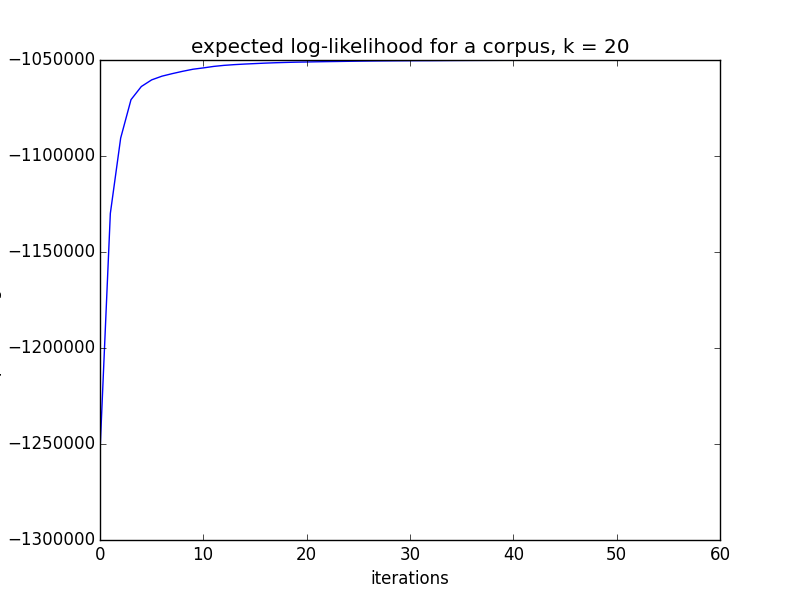
\includegraphics[width=0.5\linewidth]{../img/k=20/log_likelihood_corpus_k=20.png}
\caption{Expected log-likelihood for the corpus \texttt{reut2-000.sgm} ($k=20$)}
\label{log-likelihood-corpus}
\end{center}
\end{figure}

\begin{figure}[ht!]
\begin{center}
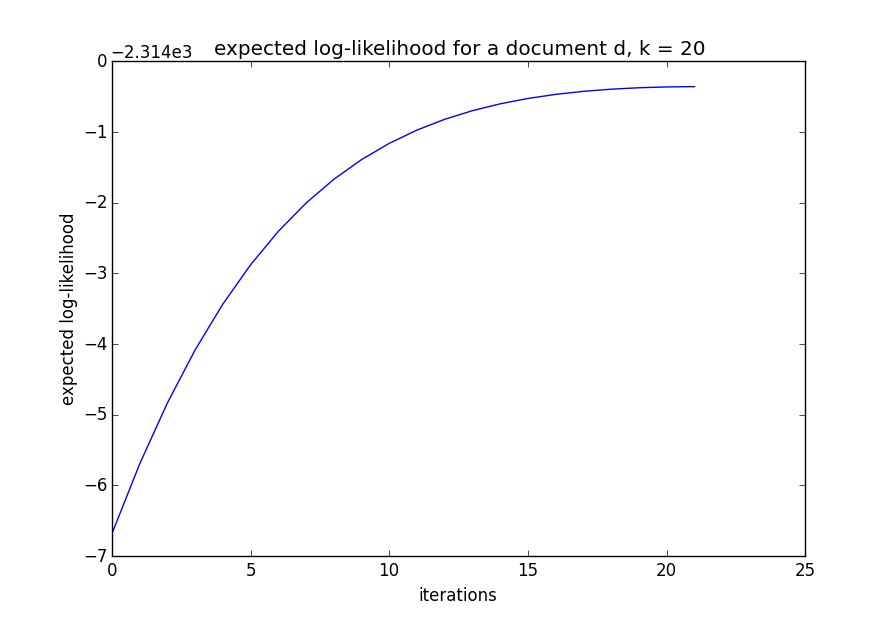
\includegraphics[width=0.5\linewidth]{../img/k=20/log_likelihood_document_k=20.png}
\caption{Expected log-likelihood for a document of the corpus \texttt{reut2-000.sgm} ($k=20$)}
\label{log-likelihood-doc}
\end{center}
\end{figure}

Multiple tries of our LDA inference program give different vectors of words for different tries. This is due to the fact that LDA inference is a non-convex optimization problem for $\alpha$ and $\beta$. The initialization of $\alpha$ and $\beta$ may infer on the final  stationary point that we get. We assumed that $\alpha$ follows the exchangeable Dirichlet distribution, which gives to the same weight to each topic.  

For $\beta$, a random initialization may give us some coherent topics (see table \ref{voc-result}). But sometimes, we obtain the same vector of words for each topic. A possible strategy to avoid that is to initialize $\beta$ differently.

\section{Document classification}

In this section, we are wondering whether the latent variables $(\gamma^{(d)}, \phi_n^{(d)})$ might be a good representation of a document $d$.

We consider the binary classification problem on a subset of the Reuters-21578 dataset (\texttt{reut2-000.sgm}, $\ldots$, \texttt{reut2-009.sgm}). The classification labels are ``\emph{earn}" and ``\emph{not earn}".

%The dataset contains 8000 documents and 15,818 words.

We trained two support vector machines (SVM) with a Gaussian RBF kernel ($\gamma= \frac{1}{2\sigma^2}=5$), using the package \texttt{scikit-learn} for Python:
\begin{itemize}
  \item one on the low-dimensional representation $\gamma^{(d)}$ provided by LDA,
  \item one on all the word features.
\end{itemize}

The accuracy rate for this binary classification problem with both representations are plotted in figure \ref{accuracy}.

\begin{figure}[ht!]
\begin{center}
%\includegraphics[width=0.5\linewidth]{../img/....png}
\caption{Accuracy rate for document classification problem}
\label{accuracy}
\end{center}
\end{figure}

Figure \ref{accuracy} shows that the LDA low-dimensional representation has a better accuracy than the ``all the word features" representation.

Topic-based representation provided by LDA may be useful as a fast filtering algorithm for feature selection in text classification.

\section{Conclusion}

LDA is an interesting way to apply graphical models to Natural Language Processing, and in our case, on information retrieval. Given a corpus and a set of vocabulary, LDA is able to group words in the same categories. The key idea in LDA is variational inference. 

There are other interesting applications of LDA, such that biology (DNA sequence), content-based image retrieval$\ldots$

\begin{thebibliography}{BNJ03}
\bibitem[BNJ03]{BNJ03} David M. Blei, Andrew Y. Ng and Michael I. Jordan. Latent Dirichlet Allocation. \emph{The Journal of Machine Learning Research}, 3:993--1022, 2003.

\bibitem[MH01]{MH01} \emph{An Experimental Comparison of Several Clustering and Initialization Methods}, Marina Meila, David Heckerman, 2001.

\bibitem[YIS]{YIS} \emph{Latent Support Measure Machines for Bag-of-Words Data Classification}, Y. Yoshikawa, T. Iwata and H. Sawada
\end{thebibliography}


\end{document}